\documentclass[14pt,letterpaper]{extarticle}
\usepackage[letterpaper,left=0.7in,right=0.7in,top=0.85in,bottom=0.85in,headheight=18pt,headsep=14pt,footskip=0.45in]{geometry}
\usepackage[T1]{fontenc}
\usepackage{newcent}
\usepackage{tikz}
\usepackage{array}
\usepackage{fancyhdr}
\pagestyle{fancy}
\fancyhf{}
\fancyhead[L]{Week 7 / Take-away games / Grades K--1}
\fancyfoot[L]{Bellingham Math Circle / Week 7}
\fancyfoot[R]{\thepage}
\renewcommand{\headrulewidth}{0.4pt}
\renewcommand{\footrulewidth}{0pt}
\setlength{\parindent}{0pt}
\setlength{\parskip}{0pt}
\newcommand{\prob}[1]{\textbf{Problem #1:}}
\newcommand{\game}[1]{\mbox{\{#1\}}}
\newenvironment{problem}{\par\noindent\begin{minipage}{\linewidth}}{\end{minipage}\par\vspace{0.9cm}}
\begin{document}
Two players take turns taking counters from a pile. On each turn, a player takes 1 counter or 2 counters. Whoever takes the last counter wins.

\vspace{0.7cm}
\begin{problem}
\prob{1} It is your turn. Circle the counters you take to be sure to win, or cross out the pile if you cannot be sure to win.
\begin{center}
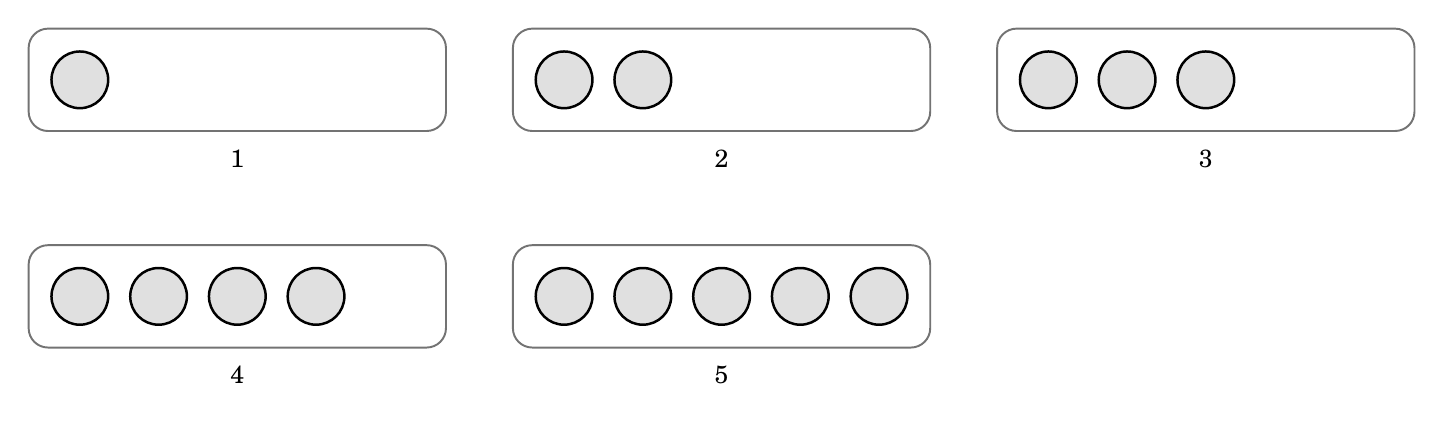
\begin{tikzpicture}
\draw[black!55,line width=0.7pt,rounded corners=7pt] (0.000,0.000) rectangle (5.300,-1.300);
\draw[fill=black!12,line width=0.9pt] (0.650,-0.650) circle (0.36);
\node[font=\small] at (2.650,-1.650) {1};
\draw[black!55,line width=0.7pt,rounded corners=7pt] (6.150,0.000) rectangle (11.450,-1.300);
\draw[fill=black!12,line width=0.9pt] (6.800,-0.650) circle (0.36);
\draw[fill=black!12,line width=0.9pt] (7.800,-0.650) circle (0.36);
\node[font=\small] at (8.800,-1.650) {2};
\draw[black!55,line width=0.7pt,rounded corners=7pt] (12.300,0.000) rectangle (17.600,-1.300);
\draw[fill=black!12,line width=0.9pt] (12.950,-0.650) circle (0.36);
\draw[fill=black!12,line width=0.9pt] (13.950,-0.650) circle (0.36);
\draw[fill=black!12,line width=0.9pt] (14.950,-0.650) circle (0.36);
\node[font=\small] at (14.950,-1.650) {3};
\draw[black!55,line width=0.7pt,rounded corners=7pt] (0.000,-2.750) rectangle (5.300,-4.050);
\draw[fill=black!12,line width=0.9pt] (0.650,-3.400) circle (0.36);
\draw[fill=black!12,line width=0.9pt] (1.650,-3.400) circle (0.36);
\draw[fill=black!12,line width=0.9pt] (2.650,-3.400) circle (0.36);
\draw[fill=black!12,line width=0.9pt] (3.650,-3.400) circle (0.36);
\node[font=\small] at (2.650,-4.400) {4};
\draw[black!55,line width=0.7pt,rounded corners=7pt] (6.150,-2.750) rectangle (11.450,-4.050);
\draw[fill=black!12,line width=0.9pt] (6.800,-3.400) circle (0.36);
\draw[fill=black!12,line width=0.9pt] (7.800,-3.400) circle (0.36);
\draw[fill=black!12,line width=0.9pt] (8.800,-3.400) circle (0.36);
\draw[fill=black!12,line width=0.9pt] (9.800,-3.400) circle (0.36);
\draw[fill=black!12,line width=0.9pt] (10.800,-3.400) circle (0.36);
\node[font=\small] at (8.800,-4.400) {5};
\end{tikzpicture}
\end{center}

\end{problem}
\begin{problem}
\prob{2} Circle 1st or 2nd to show whether you would rather go first or second with each pile.
\begin{center}
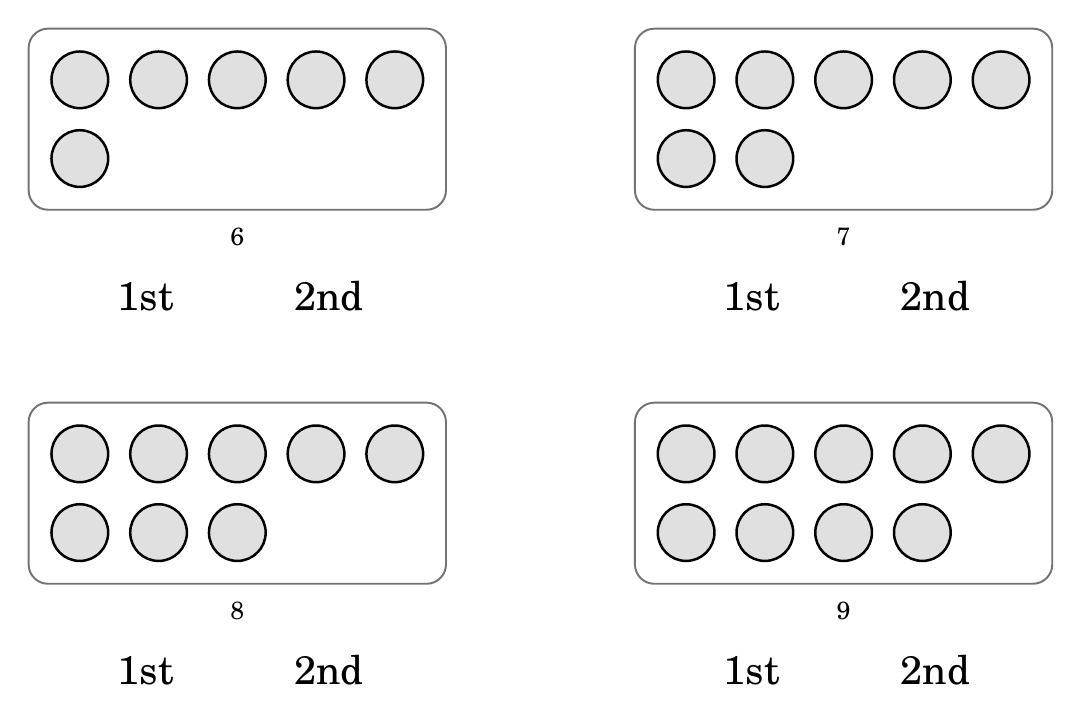
\begin{tikzpicture}
\draw[black!55,line width=0.7pt,rounded corners=7pt] (0.000,0.000) rectangle (5.300,-2.300);
\draw[fill=black!12,line width=0.9pt] (0.650,-0.650) circle (0.36);
\draw[fill=black!12,line width=0.9pt] (1.650,-0.650) circle (0.36);
\draw[fill=black!12,line width=0.9pt] (2.650,-0.650) circle (0.36);
\draw[fill=black!12,line width=0.9pt] (3.650,-0.650) circle (0.36);
\draw[fill=black!12,line width=0.9pt] (4.650,-0.650) circle (0.36);
\draw[fill=black!12,line width=0.9pt] (0.650,-1.650) circle (0.36);
\node[font=\small] at (2.650,-2.650) {6};
\node[font=\Large] at (1.484,-3.400) {1st};
\node[font=\Large] at (3.816,-3.400) {2nd};
\draw[black!55,line width=0.7pt,rounded corners=7pt] (7.700,0.000) rectangle (13.000,-2.300);
\draw[fill=black!12,line width=0.9pt] (8.350,-0.650) circle (0.36);
\draw[fill=black!12,line width=0.9pt] (9.350,-0.650) circle (0.36);
\draw[fill=black!12,line width=0.9pt] (10.350,-0.650) circle (0.36);
\draw[fill=black!12,line width=0.9pt] (11.350,-0.650) circle (0.36);
\draw[fill=black!12,line width=0.9pt] (12.350,-0.650) circle (0.36);
\draw[fill=black!12,line width=0.9pt] (8.350,-1.650) circle (0.36);
\draw[fill=black!12,line width=0.9pt] (9.350,-1.650) circle (0.36);
\node[font=\small] at (10.350,-2.650) {7};
\node[font=\Large] at (9.184,-3.400) {1st};
\node[font=\Large] at (11.516,-3.400) {2nd};
\draw[black!55,line width=0.7pt,rounded corners=7pt] (0.000,-4.750) rectangle (5.300,-7.050);
\draw[fill=black!12,line width=0.9pt] (0.650,-5.400) circle (0.36);
\draw[fill=black!12,line width=0.9pt] (1.650,-5.400) circle (0.36);
\draw[fill=black!12,line width=0.9pt] (2.650,-5.400) circle (0.36);
\draw[fill=black!12,line width=0.9pt] (3.650,-5.400) circle (0.36);
\draw[fill=black!12,line width=0.9pt] (4.650,-5.400) circle (0.36);
\draw[fill=black!12,line width=0.9pt] (0.650,-6.400) circle (0.36);
\draw[fill=black!12,line width=0.9pt] (1.650,-6.400) circle (0.36);
\draw[fill=black!12,line width=0.9pt] (2.650,-6.400) circle (0.36);
\node[font=\small] at (2.650,-7.400) {8};
\node[font=\Large] at (1.484,-8.150) {1st};
\node[font=\Large] at (3.816,-8.150) {2nd};
\draw[black!55,line width=0.7pt,rounded corners=7pt] (7.700,-4.750) rectangle (13.000,-7.050);
\draw[fill=black!12,line width=0.9pt] (8.350,-5.400) circle (0.36);
\draw[fill=black!12,line width=0.9pt] (9.350,-5.400) circle (0.36);
\draw[fill=black!12,line width=0.9pt] (10.350,-5.400) circle (0.36);
\draw[fill=black!12,line width=0.9pt] (11.350,-5.400) circle (0.36);
\draw[fill=black!12,line width=0.9pt] (12.350,-5.400) circle (0.36);
\draw[fill=black!12,line width=0.9pt] (8.350,-6.400) circle (0.36);
\draw[fill=black!12,line width=0.9pt] (9.350,-6.400) circle (0.36);
\draw[fill=black!12,line width=0.9pt] (10.350,-6.400) circle (0.36);
\draw[fill=black!12,line width=0.9pt] (11.350,-6.400) circle (0.36);
\node[font=\small] at (10.350,-7.400) {9};
\node[font=\Large] at (9.184,-8.150) {1st};
\node[font=\Large] at (11.516,-8.150) {2nd};
\end{tikzpicture}
\end{center}

\end{problem}
\begin{problem}
\prob{3} It is your turn with a bigger pile. Circle the counters you take to be sure to win, or cross out the pile if you cannot be sure to win.
\begin{center}
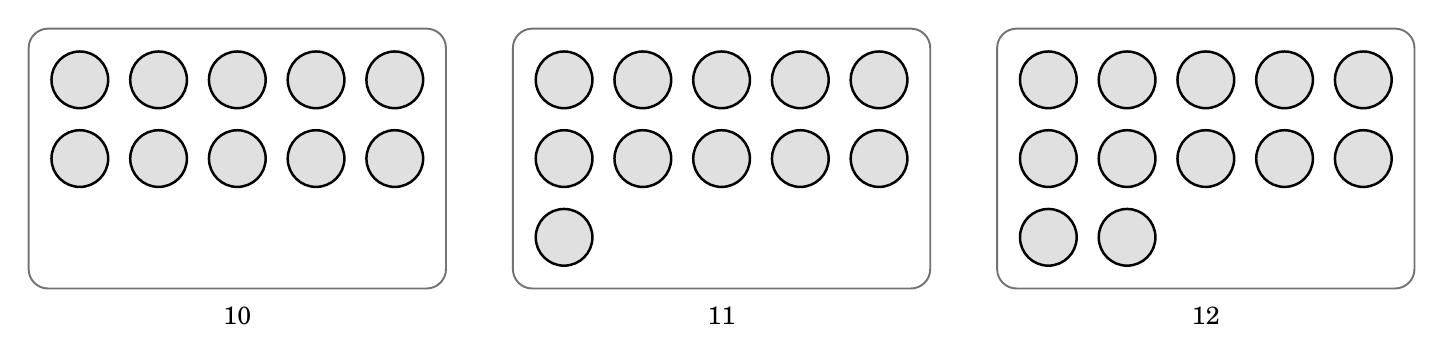
\begin{tikzpicture}
\draw[black!55,line width=0.7pt,rounded corners=7pt] (0.000,0.000) rectangle (5.300,-3.300);
\draw[fill=black!12,line width=0.9pt] (0.650,-0.650) circle (0.36);
\draw[fill=black!12,line width=0.9pt] (1.650,-0.650) circle (0.36);
\draw[fill=black!12,line width=0.9pt] (2.650,-0.650) circle (0.36);
\draw[fill=black!12,line width=0.9pt] (3.650,-0.650) circle (0.36);
\draw[fill=black!12,line width=0.9pt] (4.650,-0.650) circle (0.36);
\draw[fill=black!12,line width=0.9pt] (0.650,-1.650) circle (0.36);
\draw[fill=black!12,line width=0.9pt] (1.650,-1.650) circle (0.36);
\draw[fill=black!12,line width=0.9pt] (2.650,-1.650) circle (0.36);
\draw[fill=black!12,line width=0.9pt] (3.650,-1.650) circle (0.36);
\draw[fill=black!12,line width=0.9pt] (4.650,-1.650) circle (0.36);
\node[font=\small] at (2.650,-3.650) {10};
\draw[black!55,line width=0.7pt,rounded corners=7pt] (6.150,0.000) rectangle (11.450,-3.300);
\draw[fill=black!12,line width=0.9pt] (6.800,-0.650) circle (0.36);
\draw[fill=black!12,line width=0.9pt] (7.800,-0.650) circle (0.36);
\draw[fill=black!12,line width=0.9pt] (8.800,-0.650) circle (0.36);
\draw[fill=black!12,line width=0.9pt] (9.800,-0.650) circle (0.36);
\draw[fill=black!12,line width=0.9pt] (10.800,-0.650) circle (0.36);
\draw[fill=black!12,line width=0.9pt] (6.800,-1.650) circle (0.36);
\draw[fill=black!12,line width=0.9pt] (7.800,-1.650) circle (0.36);
\draw[fill=black!12,line width=0.9pt] (8.800,-1.650) circle (0.36);
\draw[fill=black!12,line width=0.9pt] (9.800,-1.650) circle (0.36);
\draw[fill=black!12,line width=0.9pt] (10.800,-1.650) circle (0.36);
\draw[fill=black!12,line width=0.9pt] (6.800,-2.650) circle (0.36);
\node[font=\small] at (8.800,-3.650) {11};
\draw[black!55,line width=0.7pt,rounded corners=7pt] (12.300,0.000) rectangle (17.600,-3.300);
\draw[fill=black!12,line width=0.9pt] (12.950,-0.650) circle (0.36);
\draw[fill=black!12,line width=0.9pt] (13.950,-0.650) circle (0.36);
\draw[fill=black!12,line width=0.9pt] (14.950,-0.650) circle (0.36);
\draw[fill=black!12,line width=0.9pt] (15.950,-0.650) circle (0.36);
\draw[fill=black!12,line width=0.9pt] (16.950,-0.650) circle (0.36);
\draw[fill=black!12,line width=0.9pt] (12.950,-1.650) circle (0.36);
\draw[fill=black!12,line width=0.9pt] (13.950,-1.650) circle (0.36);
\draw[fill=black!12,line width=0.9pt] (14.950,-1.650) circle (0.36);
\draw[fill=black!12,line width=0.9pt] (15.950,-1.650) circle (0.36);
\draw[fill=black!12,line width=0.9pt] (16.950,-1.650) circle (0.36);
\draw[fill=black!12,line width=0.9pt] (12.950,-2.650) circle (0.36);
\draw[fill=black!12,line width=0.9pt] (13.950,-2.650) circle (0.36);
\node[font=\small] at (14.950,-3.650) {12};
\end{tikzpicture}
\end{center}

\end{problem}
\begin{problem}
\prob{4} A pile is a trap if the player whose turn it is cannot be sure to win. Put an X on every trap from 1 to 20.
\vspace{0.2cm}
\begin{center}
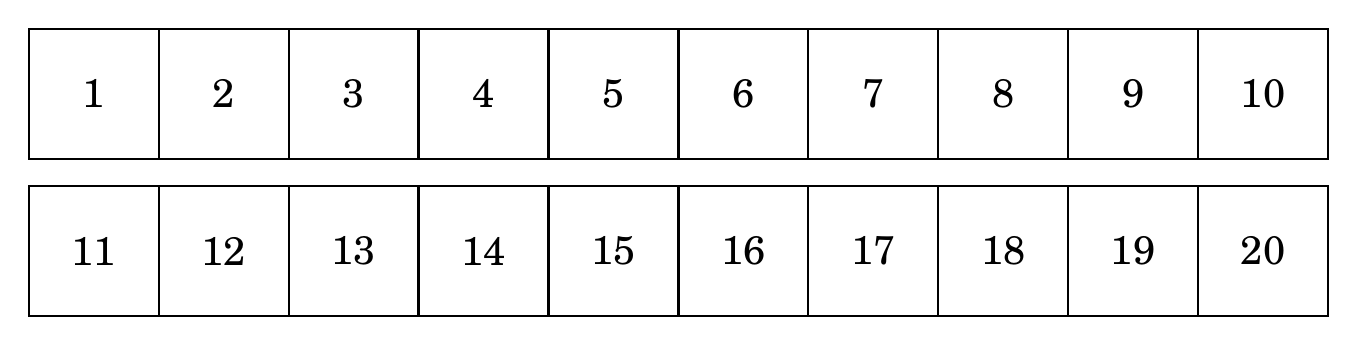
\begin{tikzpicture}
\draw[line width=0.8pt] (0.000,0.000) rectangle (1.650,-1.650);
\node[font=\Large] at (0.825,-0.825) {1};
\draw[line width=0.8pt] (1.650,0.000) rectangle (3.300,-1.650);
\node[font=\Large] at (2.475,-0.825) {2};
\draw[line width=0.8pt] (3.300,0.000) rectangle (4.950,-1.650);
\node[font=\Large] at (4.125,-0.825) {3};
\draw[line width=0.8pt] (4.950,0.000) rectangle (6.600,-1.650);
\node[font=\Large] at (5.775,-0.825) {4};
\draw[line width=0.8pt] (6.600,0.000) rectangle (8.250,-1.650);
\node[font=\Large] at (7.425,-0.825) {5};
\draw[line width=0.8pt] (8.250,0.000) rectangle (9.900,-1.650);
\node[font=\Large] at (9.075,-0.825) {6};
\draw[line width=0.8pt] (9.900,0.000) rectangle (11.550,-1.650);
\node[font=\Large] at (10.725,-0.825) {7};
\draw[line width=0.8pt] (11.550,0.000) rectangle (13.200,-1.650);
\node[font=\Large] at (12.375,-0.825) {8};
\draw[line width=0.8pt] (13.200,0.000) rectangle (14.850,-1.650);
\node[font=\Large] at (14.025,-0.825) {9};
\draw[line width=0.8pt] (14.850,0.000) rectangle (16.500,-1.650);
\node[font=\Large] at (15.675,-0.825) {10};
\draw[line width=0.8pt] (0.000,-2.000) rectangle (1.650,-3.650);
\node[font=\Large] at (0.825,-2.825) {11};
\draw[line width=0.8pt] (1.650,-2.000) rectangle (3.300,-3.650);
\node[font=\Large] at (2.475,-2.825) {12};
\draw[line width=0.8pt] (3.300,-2.000) rectangle (4.950,-3.650);
\node[font=\Large] at (4.125,-2.825) {13};
\draw[line width=0.8pt] (4.950,-2.000) rectangle (6.600,-3.650);
\node[font=\Large] at (5.775,-2.825) {14};
\draw[line width=0.8pt] (6.600,-2.000) rectangle (8.250,-3.650);
\node[font=\Large] at (7.425,-2.825) {15};
\draw[line width=0.8pt] (8.250,-2.000) rectangle (9.900,-3.650);
\node[font=\Large] at (9.075,-2.825) {16};
\draw[line width=0.8pt] (9.900,-2.000) rectangle (11.550,-3.650);
\node[font=\Large] at (10.725,-2.825) {17};
\draw[line width=0.8pt] (11.550,-2.000) rectangle (13.200,-3.650);
\node[font=\Large] at (12.375,-2.825) {18};
\draw[line width=0.8pt] (13.200,-2.000) rectangle (14.850,-3.650);
\node[font=\Large] at (14.025,-2.825) {19};
\draw[line width=0.8pt] (14.850,-2.000) rectangle (16.500,-3.650);
\node[font=\Large] at (15.675,-2.825) {20};
\end{tikzpicture}
\end{center}

\end{problem}
\begin{problem}
\prob{5} Ben always starts by taking 2 counters. Circle each pile where Ben can still be sure to win after that.
\begin{center}
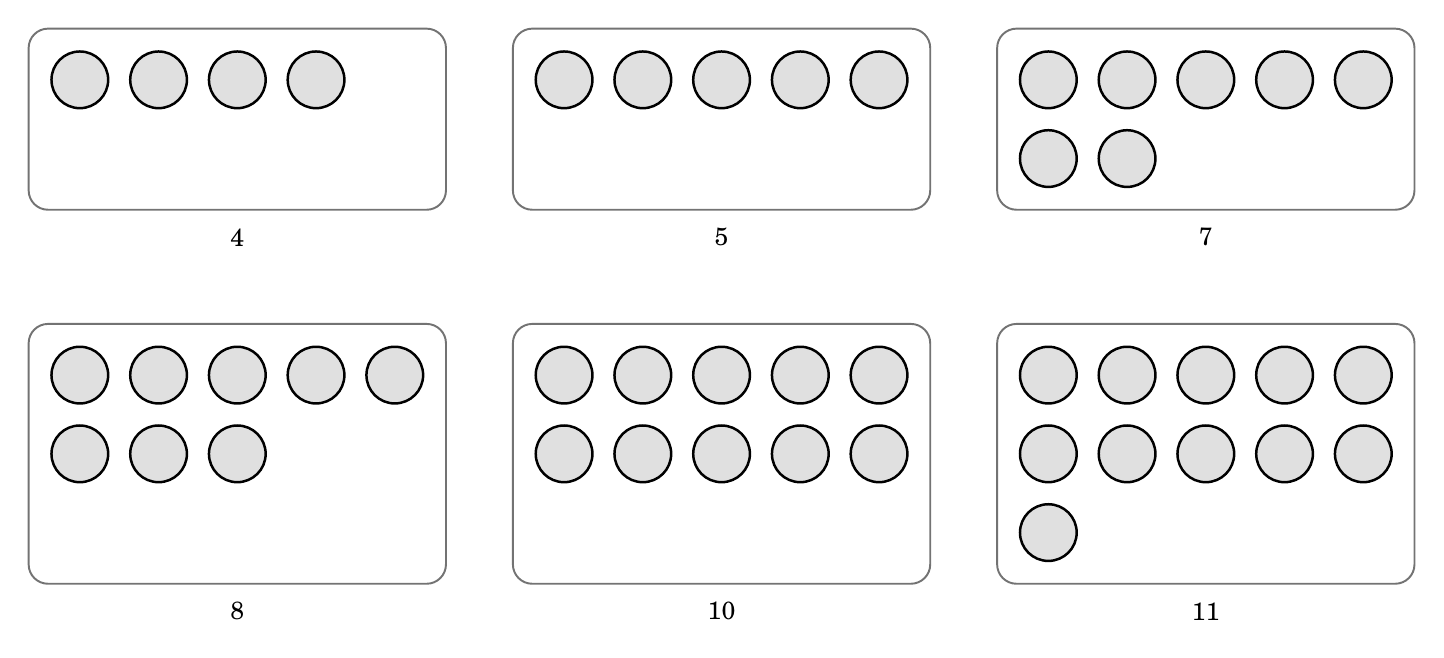
\begin{tikzpicture}
\draw[black!55,line width=0.7pt,rounded corners=7pt] (0.000,0.000) rectangle (5.300,-2.300);
\draw[fill=black!12,line width=0.9pt] (0.650,-0.650) circle (0.36);
\draw[fill=black!12,line width=0.9pt] (1.650,-0.650) circle (0.36);
\draw[fill=black!12,line width=0.9pt] (2.650,-0.650) circle (0.36);
\draw[fill=black!12,line width=0.9pt] (3.650,-0.650) circle (0.36);
\node[font=\small] at (2.650,-2.650) {4};
\draw[black!55,line width=0.7pt,rounded corners=7pt] (6.150,0.000) rectangle (11.450,-2.300);
\draw[fill=black!12,line width=0.9pt] (6.800,-0.650) circle (0.36);
\draw[fill=black!12,line width=0.9pt] (7.800,-0.650) circle (0.36);
\draw[fill=black!12,line width=0.9pt] (8.800,-0.650) circle (0.36);
\draw[fill=black!12,line width=0.9pt] (9.800,-0.650) circle (0.36);
\draw[fill=black!12,line width=0.9pt] (10.800,-0.650) circle (0.36);
\node[font=\small] at (8.800,-2.650) {5};
\draw[black!55,line width=0.7pt,rounded corners=7pt] (12.300,0.000) rectangle (17.600,-2.300);
\draw[fill=black!12,line width=0.9pt] (12.950,-0.650) circle (0.36);
\draw[fill=black!12,line width=0.9pt] (13.950,-0.650) circle (0.36);
\draw[fill=black!12,line width=0.9pt] (14.950,-0.650) circle (0.36);
\draw[fill=black!12,line width=0.9pt] (15.950,-0.650) circle (0.36);
\draw[fill=black!12,line width=0.9pt] (16.950,-0.650) circle (0.36);
\draw[fill=black!12,line width=0.9pt] (12.950,-1.650) circle (0.36);
\draw[fill=black!12,line width=0.9pt] (13.950,-1.650) circle (0.36);
\node[font=\small] at (14.950,-2.650) {7};
\draw[black!55,line width=0.7pt,rounded corners=7pt] (0.000,-3.750) rectangle (5.300,-7.050);
\draw[fill=black!12,line width=0.9pt] (0.650,-4.400) circle (0.36);
\draw[fill=black!12,line width=0.9pt] (1.650,-4.400) circle (0.36);
\draw[fill=black!12,line width=0.9pt] (2.650,-4.400) circle (0.36);
\draw[fill=black!12,line width=0.9pt] (3.650,-4.400) circle (0.36);
\draw[fill=black!12,line width=0.9pt] (4.650,-4.400) circle (0.36);
\draw[fill=black!12,line width=0.9pt] (0.650,-5.400) circle (0.36);
\draw[fill=black!12,line width=0.9pt] (1.650,-5.400) circle (0.36);
\draw[fill=black!12,line width=0.9pt] (2.650,-5.400) circle (0.36);
\node[font=\small] at (2.650,-7.400) {8};
\draw[black!55,line width=0.7pt,rounded corners=7pt] (6.150,-3.750) rectangle (11.450,-7.050);
\draw[fill=black!12,line width=0.9pt] (6.800,-4.400) circle (0.36);
\draw[fill=black!12,line width=0.9pt] (7.800,-4.400) circle (0.36);
\draw[fill=black!12,line width=0.9pt] (8.800,-4.400) circle (0.36);
\draw[fill=black!12,line width=0.9pt] (9.800,-4.400) circle (0.36);
\draw[fill=black!12,line width=0.9pt] (10.800,-4.400) circle (0.36);
\draw[fill=black!12,line width=0.9pt] (6.800,-5.400) circle (0.36);
\draw[fill=black!12,line width=0.9pt] (7.800,-5.400) circle (0.36);
\draw[fill=black!12,line width=0.9pt] (8.800,-5.400) circle (0.36);
\draw[fill=black!12,line width=0.9pt] (9.800,-5.400) circle (0.36);
\draw[fill=black!12,line width=0.9pt] (10.800,-5.400) circle (0.36);
\node[font=\small] at (8.800,-7.400) {10};
\draw[black!55,line width=0.7pt,rounded corners=7pt] (12.300,-3.750) rectangle (17.600,-7.050);
\draw[fill=black!12,line width=0.9pt] (12.950,-4.400) circle (0.36);
\draw[fill=black!12,line width=0.9pt] (13.950,-4.400) circle (0.36);
\draw[fill=black!12,line width=0.9pt] (14.950,-4.400) circle (0.36);
\draw[fill=black!12,line width=0.9pt] (15.950,-4.400) circle (0.36);
\draw[fill=black!12,line width=0.9pt] (16.950,-4.400) circle (0.36);
\draw[fill=black!12,line width=0.9pt] (12.950,-5.400) circle (0.36);
\draw[fill=black!12,line width=0.9pt] (13.950,-5.400) circle (0.36);
\draw[fill=black!12,line width=0.9pt] (14.950,-5.400) circle (0.36);
\draw[fill=black!12,line width=0.9pt] (15.950,-5.400) circle (0.36);
\draw[fill=black!12,line width=0.9pt] (16.950,-5.400) circle (0.36);
\draw[fill=black!12,line width=0.9pt] (12.950,-6.400) circle (0.36);
\node[font=\small] at (14.950,-7.400) {11};
\end{tikzpicture}
\end{center}

\end{problem}
\begin{problem}
\prob{6} Show every different way a game with 4 counters can go, and then every way a game with 5 counters can go. Circle the counters taken on each turn.
\vspace{0.3cm}
\begin{center}
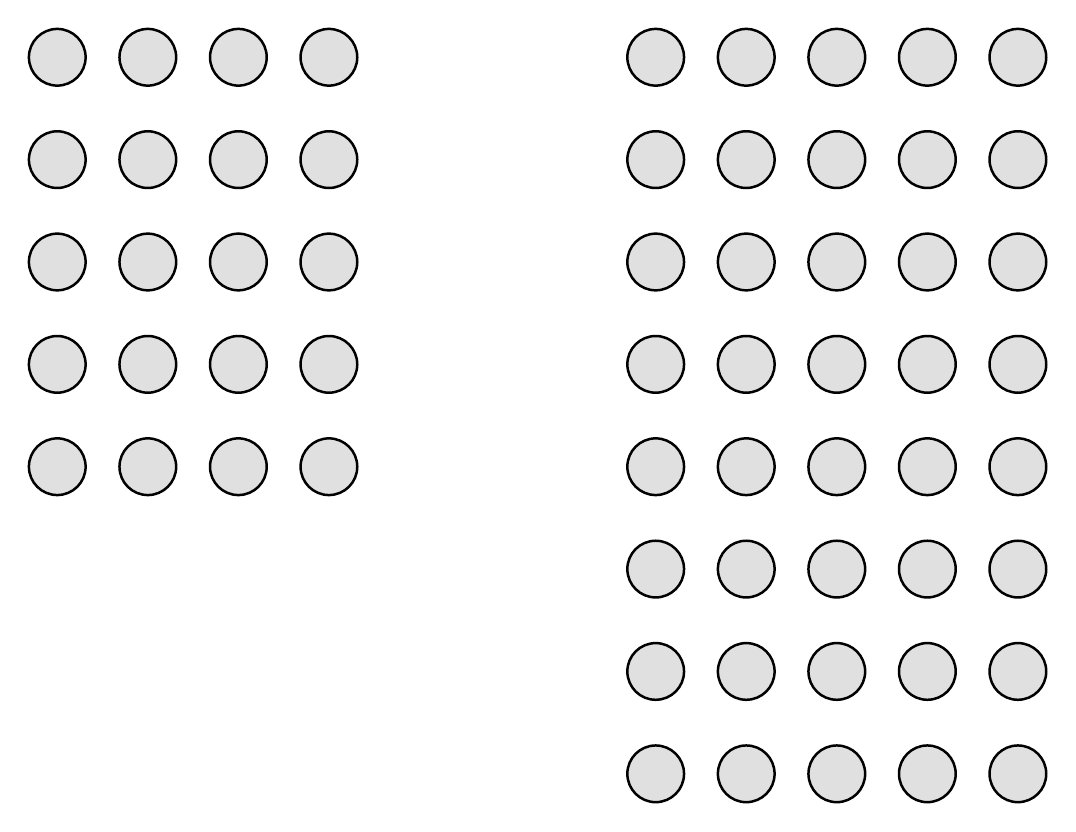
\begin{tikzpicture}
\draw[fill=black!12,line width=0.9pt] (0.000,0.000) circle (0.36);
\draw[fill=black!12,line width=0.9pt] (1.150,0.000) circle (0.36);
\draw[fill=black!12,line width=0.9pt] (2.300,0.000) circle (0.36);
\draw[fill=black!12,line width=0.9pt] (3.450,0.000) circle (0.36);
\draw[fill=black!12,line width=0.9pt] (0.000,-1.300) circle (0.36);
\draw[fill=black!12,line width=0.9pt] (1.150,-1.300) circle (0.36);
\draw[fill=black!12,line width=0.9pt] (2.300,-1.300) circle (0.36);
\draw[fill=black!12,line width=0.9pt] (3.450,-1.300) circle (0.36);
\draw[fill=black!12,line width=0.9pt] (0.000,-2.600) circle (0.36);
\draw[fill=black!12,line width=0.9pt] (1.150,-2.600) circle (0.36);
\draw[fill=black!12,line width=0.9pt] (2.300,-2.600) circle (0.36);
\draw[fill=black!12,line width=0.9pt] (3.450,-2.600) circle (0.36);
\draw[fill=black!12,line width=0.9pt] (0.000,-3.900) circle (0.36);
\draw[fill=black!12,line width=0.9pt] (1.150,-3.900) circle (0.36);
\draw[fill=black!12,line width=0.9pt] (2.300,-3.900) circle (0.36);
\draw[fill=black!12,line width=0.9pt] (3.450,-3.900) circle (0.36);
\draw[fill=black!12,line width=0.9pt] (0.000,-5.200) circle (0.36);
\draw[fill=black!12,line width=0.9pt] (1.150,-5.200) circle (0.36);
\draw[fill=black!12,line width=0.9pt] (2.300,-5.200) circle (0.36);
\draw[fill=black!12,line width=0.9pt] (3.450,-5.200) circle (0.36);
\draw[fill=black!12,line width=0.9pt] (7.600,0.000) circle (0.36);
\draw[fill=black!12,line width=0.9pt] (8.750,0.000) circle (0.36);
\draw[fill=black!12,line width=0.9pt] (9.900,0.000) circle (0.36);
\draw[fill=black!12,line width=0.9pt] (11.050,0.000) circle (0.36);
\draw[fill=black!12,line width=0.9pt] (12.200,0.000) circle (0.36);
\draw[fill=black!12,line width=0.9pt] (7.600,-1.300) circle (0.36);
\draw[fill=black!12,line width=0.9pt] (8.750,-1.300) circle (0.36);
\draw[fill=black!12,line width=0.9pt] (9.900,-1.300) circle (0.36);
\draw[fill=black!12,line width=0.9pt] (11.050,-1.300) circle (0.36);
\draw[fill=black!12,line width=0.9pt] (12.200,-1.300) circle (0.36);
\draw[fill=black!12,line width=0.9pt] (7.600,-2.600) circle (0.36);
\draw[fill=black!12,line width=0.9pt] (8.750,-2.600) circle (0.36);
\draw[fill=black!12,line width=0.9pt] (9.900,-2.600) circle (0.36);
\draw[fill=black!12,line width=0.9pt] (11.050,-2.600) circle (0.36);
\draw[fill=black!12,line width=0.9pt] (12.200,-2.600) circle (0.36);
\draw[fill=black!12,line width=0.9pt] (7.600,-3.900) circle (0.36);
\draw[fill=black!12,line width=0.9pt] (8.750,-3.900) circle (0.36);
\draw[fill=black!12,line width=0.9pt] (9.900,-3.900) circle (0.36);
\draw[fill=black!12,line width=0.9pt] (11.050,-3.900) circle (0.36);
\draw[fill=black!12,line width=0.9pt] (12.200,-3.900) circle (0.36);
\draw[fill=black!12,line width=0.9pt] (7.600,-5.200) circle (0.36);
\draw[fill=black!12,line width=0.9pt] (8.750,-5.200) circle (0.36);
\draw[fill=black!12,line width=0.9pt] (9.900,-5.200) circle (0.36);
\draw[fill=black!12,line width=0.9pt] (11.050,-5.200) circle (0.36);
\draw[fill=black!12,line width=0.9pt] (12.200,-5.200) circle (0.36);
\draw[fill=black!12,line width=0.9pt] (7.600,-6.500) circle (0.36);
\draw[fill=black!12,line width=0.9pt] (8.750,-6.500) circle (0.36);
\draw[fill=black!12,line width=0.9pt] (9.900,-6.500) circle (0.36);
\draw[fill=black!12,line width=0.9pt] (11.050,-6.500) circle (0.36);
\draw[fill=black!12,line width=0.9pt] (12.200,-6.500) circle (0.36);
\draw[fill=black!12,line width=0.9pt] (7.600,-7.800) circle (0.36);
\draw[fill=black!12,line width=0.9pt] (8.750,-7.800) circle (0.36);
\draw[fill=black!12,line width=0.9pt] (9.900,-7.800) circle (0.36);
\draw[fill=black!12,line width=0.9pt] (11.050,-7.800) circle (0.36);
\draw[fill=black!12,line width=0.9pt] (12.200,-7.800) circle (0.36);
\draw[fill=black!12,line width=0.9pt] (7.600,-9.100) circle (0.36);
\draw[fill=black!12,line width=0.9pt] (8.750,-9.100) circle (0.36);
\draw[fill=black!12,line width=0.9pt] (9.900,-9.100) circle (0.36);
\draw[fill=black!12,line width=0.9pt] (11.050,-9.100) circle (0.36);
\draw[fill=black!12,line width=0.9pt] (12.200,-9.100) circle (0.36);
\end{tikzpicture}
\end{center}

\end{problem}
\begin{problem}
\prob{7} Now each player may take 1, 2, or 3 counters on a turn. Put an X on every trap from 1 to 20.
\vspace{0.2cm}
\begin{center}
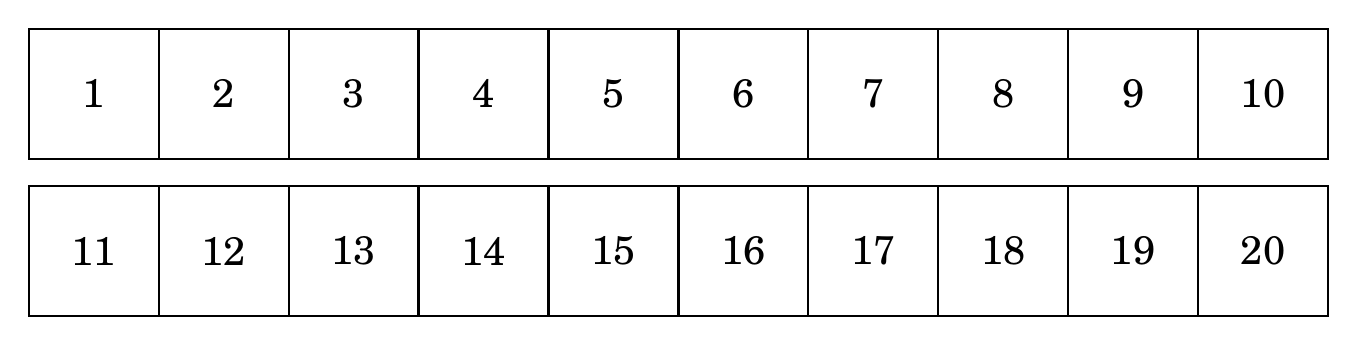
\begin{tikzpicture}
\draw[line width=0.8pt] (0.000,0.000) rectangle (1.650,-1.650);
\node[font=\Large] at (0.825,-0.825) {1};
\draw[line width=0.8pt] (1.650,0.000) rectangle (3.300,-1.650);
\node[font=\Large] at (2.475,-0.825) {2};
\draw[line width=0.8pt] (3.300,0.000) rectangle (4.950,-1.650);
\node[font=\Large] at (4.125,-0.825) {3};
\draw[line width=0.8pt] (4.950,0.000) rectangle (6.600,-1.650);
\node[font=\Large] at (5.775,-0.825) {4};
\draw[line width=0.8pt] (6.600,0.000) rectangle (8.250,-1.650);
\node[font=\Large] at (7.425,-0.825) {5};
\draw[line width=0.8pt] (8.250,0.000) rectangle (9.900,-1.650);
\node[font=\Large] at (9.075,-0.825) {6};
\draw[line width=0.8pt] (9.900,0.000) rectangle (11.550,-1.650);
\node[font=\Large] at (10.725,-0.825) {7};
\draw[line width=0.8pt] (11.550,0.000) rectangle (13.200,-1.650);
\node[font=\Large] at (12.375,-0.825) {8};
\draw[line width=0.8pt] (13.200,0.000) rectangle (14.850,-1.650);
\node[font=\Large] at (14.025,-0.825) {9};
\draw[line width=0.8pt] (14.850,0.000) rectangle (16.500,-1.650);
\node[font=\Large] at (15.675,-0.825) {10};
\draw[line width=0.8pt] (0.000,-2.000) rectangle (1.650,-3.650);
\node[font=\Large] at (0.825,-2.825) {11};
\draw[line width=0.8pt] (1.650,-2.000) rectangle (3.300,-3.650);
\node[font=\Large] at (2.475,-2.825) {12};
\draw[line width=0.8pt] (3.300,-2.000) rectangle (4.950,-3.650);
\node[font=\Large] at (4.125,-2.825) {13};
\draw[line width=0.8pt] (4.950,-2.000) rectangle (6.600,-3.650);
\node[font=\Large] at (5.775,-2.825) {14};
\draw[line width=0.8pt] (6.600,-2.000) rectangle (8.250,-3.650);
\node[font=\Large] at (7.425,-2.825) {15};
\draw[line width=0.8pt] (8.250,-2.000) rectangle (9.900,-3.650);
\node[font=\Large] at (9.075,-2.825) {16};
\draw[line width=0.8pt] (9.900,-2.000) rectangle (11.550,-3.650);
\node[font=\Large] at (10.725,-2.825) {17};
\draw[line width=0.8pt] (11.550,-2.000) rectangle (13.200,-3.650);
\node[font=\Large] at (12.375,-2.825) {18};
\draw[line width=0.8pt] (13.200,-2.000) rectangle (14.850,-3.650);
\node[font=\Large] at (14.025,-2.825) {19};
\draw[line width=0.8pt] (14.850,-2.000) rectangle (16.500,-3.650);
\node[font=\Large] at (15.675,-2.825) {20};
\end{tikzpicture}
\end{center}

\end{problem}
\begin{problem}
\prob{8} Now there are two piles, and on your turn you take 1 or 2 counters from one pile. Whoever takes the last counter on the table wins. Circle 1st or 2nd to show whether you would rather go first or second.
\begin{center}
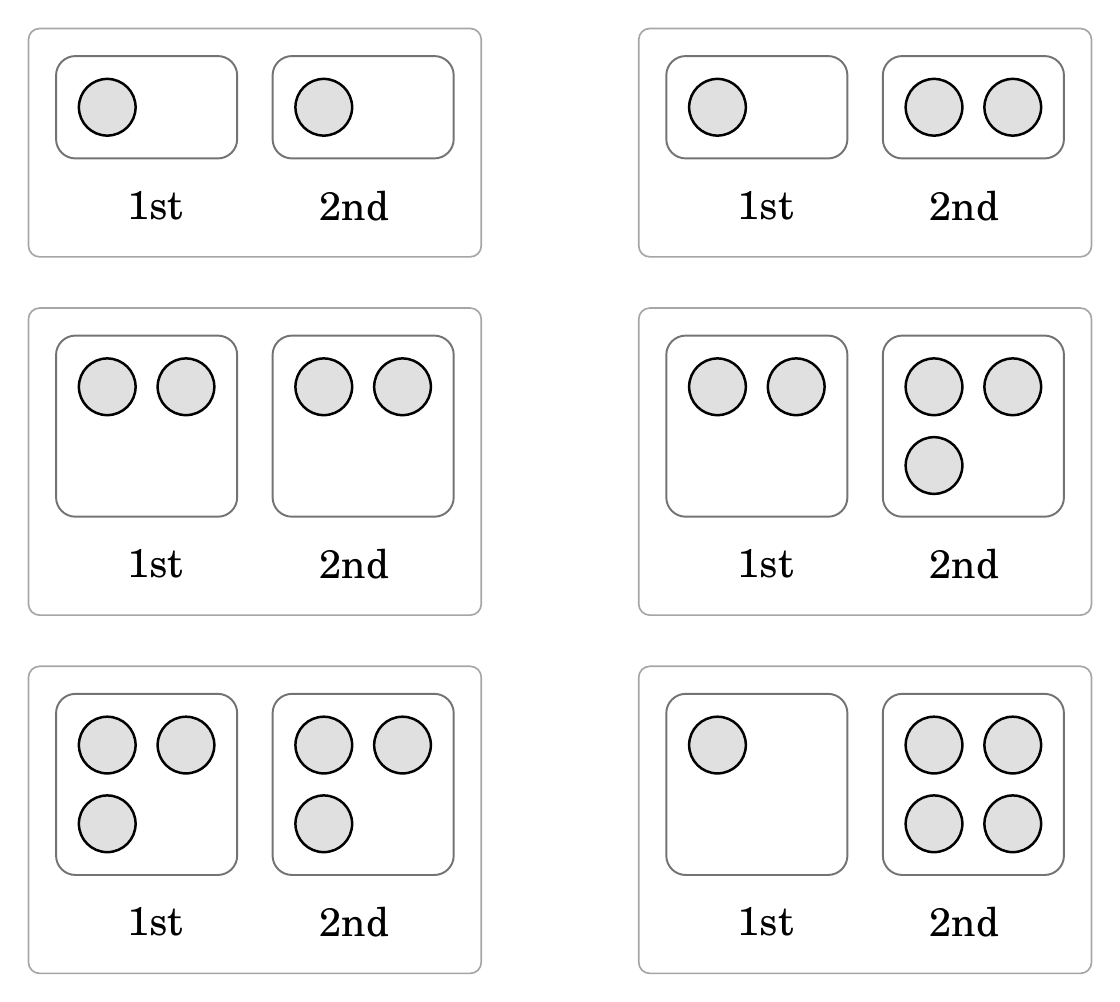
\begin{tikzpicture}
\draw[black!55,line width=0.7pt,rounded corners=7pt] (0.000,0.000) rectangle (2.300,-1.300);
\draw[fill=black!12,line width=0.9pt] (0.650,-0.650) circle (0.36);
\draw[black!55,line width=0.7pt,rounded corners=7pt] (2.750,0.000) rectangle (5.050,-1.300);
\draw[fill=black!12,line width=0.9pt] (3.400,-0.650) circle (0.36);
\node[font=\Large] at (1.262,-1.900) {1st};
\node[font=\Large] at (3.787,-1.900) {2nd};
\draw[black!35,line width=0.6pt,rounded corners=4pt] (-0.350,0.350) rectangle (5.400,-2.550);
\draw[black!55,line width=0.7pt,rounded corners=7pt] (7.750,0.000) rectangle (10.050,-1.300);
\draw[fill=black!12,line width=0.9pt] (8.400,-0.650) circle (0.36);
\draw[black!55,line width=0.7pt,rounded corners=7pt] (10.500,0.000) rectangle (12.800,-1.300);
\draw[fill=black!12,line width=0.9pt] (11.150,-0.650) circle (0.36);
\draw[fill=black!12,line width=0.9pt] (12.150,-0.650) circle (0.36);
\node[font=\Large] at (9.012,-1.900) {1st};
\node[font=\Large] at (11.537,-1.900) {2nd};
\draw[black!35,line width=0.6pt,rounded corners=4pt] (7.400,0.350) rectangle (13.150,-2.550);
\draw[black!55,line width=0.7pt,rounded corners=7pt] (0.000,-3.550) rectangle (2.300,-5.850);
\draw[fill=black!12,line width=0.9pt] (0.650,-4.200) circle (0.36);
\draw[fill=black!12,line width=0.9pt] (1.650,-4.200) circle (0.36);
\draw[black!55,line width=0.7pt,rounded corners=7pt] (2.750,-3.550) rectangle (5.050,-5.850);
\draw[fill=black!12,line width=0.9pt] (3.400,-4.200) circle (0.36);
\draw[fill=black!12,line width=0.9pt] (4.400,-4.200) circle (0.36);
\node[font=\Large] at (1.262,-6.450) {1st};
\node[font=\Large] at (3.787,-6.450) {2nd};
\draw[black!35,line width=0.6pt,rounded corners=4pt] (-0.350,-3.200) rectangle (5.400,-7.100);
\draw[black!55,line width=0.7pt,rounded corners=7pt] (7.750,-3.550) rectangle (10.050,-5.850);
\draw[fill=black!12,line width=0.9pt] (8.400,-4.200) circle (0.36);
\draw[fill=black!12,line width=0.9pt] (9.400,-4.200) circle (0.36);
\draw[black!55,line width=0.7pt,rounded corners=7pt] (10.500,-3.550) rectangle (12.800,-5.850);
\draw[fill=black!12,line width=0.9pt] (11.150,-4.200) circle (0.36);
\draw[fill=black!12,line width=0.9pt] (12.150,-4.200) circle (0.36);
\draw[fill=black!12,line width=0.9pt] (11.150,-5.200) circle (0.36);
\node[font=\Large] at (9.012,-6.450) {1st};
\node[font=\Large] at (11.537,-6.450) {2nd};
\draw[black!35,line width=0.6pt,rounded corners=4pt] (7.400,-3.200) rectangle (13.150,-7.100);
\draw[black!55,line width=0.7pt,rounded corners=7pt] (0.000,-8.100) rectangle (2.300,-10.400);
\draw[fill=black!12,line width=0.9pt] (0.650,-8.750) circle (0.36);
\draw[fill=black!12,line width=0.9pt] (1.650,-8.750) circle (0.36);
\draw[fill=black!12,line width=0.9pt] (0.650,-9.750) circle (0.36);
\draw[black!55,line width=0.7pt,rounded corners=7pt] (2.750,-8.100) rectangle (5.050,-10.400);
\draw[fill=black!12,line width=0.9pt] (3.400,-8.750) circle (0.36);
\draw[fill=black!12,line width=0.9pt] (4.400,-8.750) circle (0.36);
\draw[fill=black!12,line width=0.9pt] (3.400,-9.750) circle (0.36);
\node[font=\Large] at (1.262,-11.000) {1st};
\node[font=\Large] at (3.787,-11.000) {2nd};
\draw[black!35,line width=0.6pt,rounded corners=4pt] (-0.350,-7.750) rectangle (5.400,-11.650);
\draw[black!55,line width=0.7pt,rounded corners=7pt] (7.750,-8.100) rectangle (10.050,-10.400);
\draw[fill=black!12,line width=0.9pt] (8.400,-8.750) circle (0.36);
\draw[black!55,line width=0.7pt,rounded corners=7pt] (10.500,-8.100) rectangle (12.800,-10.400);
\draw[fill=black!12,line width=0.9pt] (11.150,-8.750) circle (0.36);
\draw[fill=black!12,line width=0.9pt] (12.150,-8.750) circle (0.36);
\draw[fill=black!12,line width=0.9pt] (11.150,-9.750) circle (0.36);
\draw[fill=black!12,line width=0.9pt] (12.150,-9.750) circle (0.36);
\node[font=\Large] at (9.012,-11.000) {1st};
\node[font=\Large] at (11.537,-11.000) {2nd};
\draw[black!35,line width=0.6pt,rounded corners=4pt] (7.400,-7.750) rectangle (13.150,-11.650);
\end{tikzpicture}
\end{center}

\end{problem}
\begin{problem}
\prob{9} Play the game from Problem 8 with two piles of 6 counters. If you go second, how can you win every time, whatever the other player does?
\begin{center}
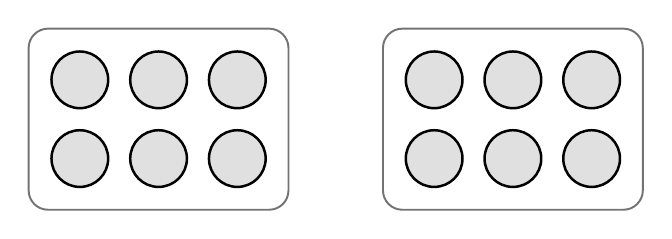
\begin{tikzpicture}
\draw[black!55,line width=0.7pt,rounded corners=7pt] (0.000,0.000) rectangle (3.300,-2.300);
\draw[fill=black!12,line width=0.9pt] (0.650,-0.650) circle (0.36);
\draw[fill=black!12,line width=0.9pt] (1.650,-0.650) circle (0.36);
\draw[fill=black!12,line width=0.9pt] (2.650,-0.650) circle (0.36);
\draw[fill=black!12,line width=0.9pt] (0.650,-1.650) circle (0.36);
\draw[fill=black!12,line width=0.9pt] (1.650,-1.650) circle (0.36);
\draw[fill=black!12,line width=0.9pt] (2.650,-1.650) circle (0.36);
\draw[black!55,line width=0.7pt,rounded corners=7pt] (4.500,0.000) rectangle (7.800,-2.300);
\draw[fill=black!12,line width=0.9pt] (5.150,-0.650) circle (0.36);
\draw[fill=black!12,line width=0.9pt] (6.150,-0.650) circle (0.36);
\draw[fill=black!12,line width=0.9pt] (7.150,-0.650) circle (0.36);
\draw[fill=black!12,line width=0.9pt] (5.150,-1.650) circle (0.36);
\draw[fill=black!12,line width=0.9pt] (6.150,-1.650) circle (0.36);
\draw[fill=black!12,line width=0.9pt] (7.150,-1.650) circle (0.36);
\end{tikzpicture}
\end{center}

\end{problem}
\begin{problem}
\prob{10} Now there is one pile again, and whoever takes the last counter loses. Each player may take 1 or 2 counters on a turn. Put an X on every trap from 1 to 20.
\vspace{0.2cm}
\begin{center}
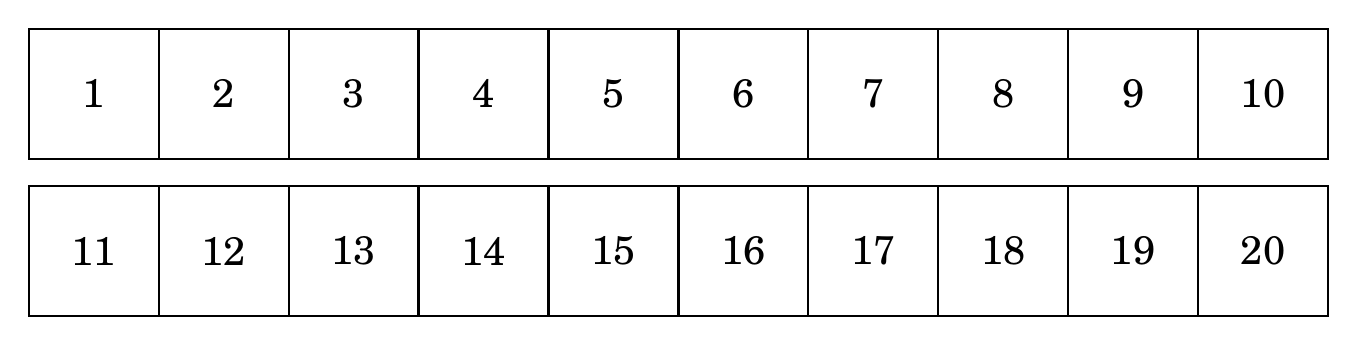
\begin{tikzpicture}
\draw[line width=0.8pt] (0.000,0.000) rectangle (1.650,-1.650);
\node[font=\Large] at (0.825,-0.825) {1};
\draw[line width=0.8pt] (1.650,0.000) rectangle (3.300,-1.650);
\node[font=\Large] at (2.475,-0.825) {2};
\draw[line width=0.8pt] (3.300,0.000) rectangle (4.950,-1.650);
\node[font=\Large] at (4.125,-0.825) {3};
\draw[line width=0.8pt] (4.950,0.000) rectangle (6.600,-1.650);
\node[font=\Large] at (5.775,-0.825) {4};
\draw[line width=0.8pt] (6.600,0.000) rectangle (8.250,-1.650);
\node[font=\Large] at (7.425,-0.825) {5};
\draw[line width=0.8pt] (8.250,0.000) rectangle (9.900,-1.650);
\node[font=\Large] at (9.075,-0.825) {6};
\draw[line width=0.8pt] (9.900,0.000) rectangle (11.550,-1.650);
\node[font=\Large] at (10.725,-0.825) {7};
\draw[line width=0.8pt] (11.550,0.000) rectangle (13.200,-1.650);
\node[font=\Large] at (12.375,-0.825) {8};
\draw[line width=0.8pt] (13.200,0.000) rectangle (14.850,-1.650);
\node[font=\Large] at (14.025,-0.825) {9};
\draw[line width=0.8pt] (14.850,0.000) rectangle (16.500,-1.650);
\node[font=\Large] at (15.675,-0.825) {10};
\draw[line width=0.8pt] (0.000,-2.000) rectangle (1.650,-3.650);
\node[font=\Large] at (0.825,-2.825) {11};
\draw[line width=0.8pt] (1.650,-2.000) rectangle (3.300,-3.650);
\node[font=\Large] at (2.475,-2.825) {12};
\draw[line width=0.8pt] (3.300,-2.000) rectangle (4.950,-3.650);
\node[font=\Large] at (4.125,-2.825) {13};
\draw[line width=0.8pt] (4.950,-2.000) rectangle (6.600,-3.650);
\node[font=\Large] at (5.775,-2.825) {14};
\draw[line width=0.8pt] (6.600,-2.000) rectangle (8.250,-3.650);
\node[font=\Large] at (7.425,-2.825) {15};
\draw[line width=0.8pt] (8.250,-2.000) rectangle (9.900,-3.650);
\node[font=\Large] at (9.075,-2.825) {16};
\draw[line width=0.8pt] (9.900,-2.000) rectangle (11.550,-3.650);
\node[font=\Large] at (10.725,-2.825) {17};
\draw[line width=0.8pt] (11.550,-2.000) rectangle (13.200,-3.650);
\node[font=\Large] at (12.375,-2.825) {18};
\draw[line width=0.8pt] (13.200,-2.000) rectangle (14.850,-3.650);
\node[font=\Large] at (14.025,-2.825) {19};
\draw[line width=0.8pt] (14.850,-2.000) rectangle (16.500,-3.650);
\node[font=\Large] at (15.675,-2.825) {20};
\end{tikzpicture}
\end{center}

\end{problem}
\end{document}
